\section{Discussion}
\label{chap:Discussion}

\subsection{Part A}
\label{chap:PartA}

\subsubsection{Ordinary Least Squares, Ridge regression and Stochastic Gradient Descent on terrain's heights GeoTIF image-data}
\label{chap:Ordinary Least Squares, Ridge regression and Stochastic Gradient Descent on terrain's heights GeoTIF image-data}

\qquad \, We start part A of this project with a re-capitulation of \href{https://github.com/fabiorodp/UiO-FYS-STK4155/blob/master/Project1}{Project 1}, part F and G, where a GeoTIF terrain image, containing the heights of a region near Stavanger/Norway, was extracted and examined on Ordinary Least Squares (OLS) and Ridge regression models. On that occasion, we generated two sets of explanatory variables ($\boldsymbol{x1}$, $\boldsymbol{x2}$), with values between 0 and 1, and utilized them on the design matrix ($\boldsymbol{X}$) function that performed a polynomial transformation with a degree equals 10 for OLS and 11 for Ridge. The response variable set ($\boldsymbol{z}$) had space (number of samples or size of the sliced image) of 15 (15x15 pixels). Lastly, the testing MSE (mean squared error) scores obtained were 1.11 and 1.44 for OLS and Ridge, respectively.\\

Now, we perform a Stochastic Gradient Descent (SGD) utilizing the same generated data as above. It is essential to say that we do not scale the data-sets because of possible crashes during the gradient computations. The \href{https://github.com/fabiorodp/UiO-FYS-STK4155/blob/master/Project2/package/gradient_descent.py}{gradient\_descent.py} under the \href{https://github.com/fabiorodp/UiO-FYS-STK4155/tree/master/Project2/package}{Project2/package/} directory has the algorithms for GDM and Mini-SGDM.\\

Our first experiment for SGD is a Grid-Search, also incorporated at the \href{https://github.com/fabiorodp/UiO-FYS-STK4155/tree/master/Project2/package}{Project2/package/} directory with the file name \href{https://github.com/fabiorodp/UiO-FYS-STK4155/blob/master/Project2/package/grid_search.py}{grid\_search.py}. We run the Grid-Search class to find the best constant learning rate ($\eta$ = [0.02, 0.01, 0.005, 0.001, 0.0005]) as function of the number of interactions (epochs=[100, 500, 1000, 5000, 10000]). The model applied to the Grid-Search is the MiniSGDM class, which is an SGD when the number of batches is equal to 1, gamma=0, lambda=0, and decay=0.\\

The results are as follows:

\begin{figure}[H]
\label{fig:figA1}
\centering
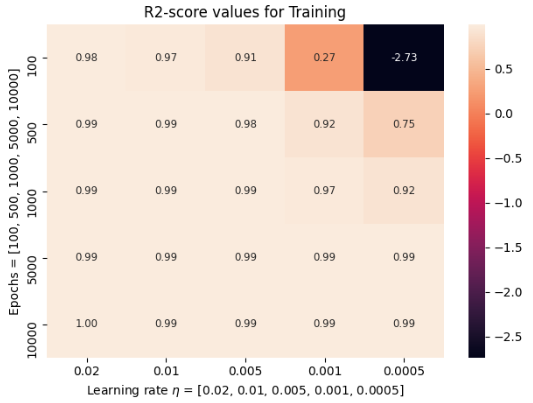
\includegraphics[width=7cm]{heatmapA1}
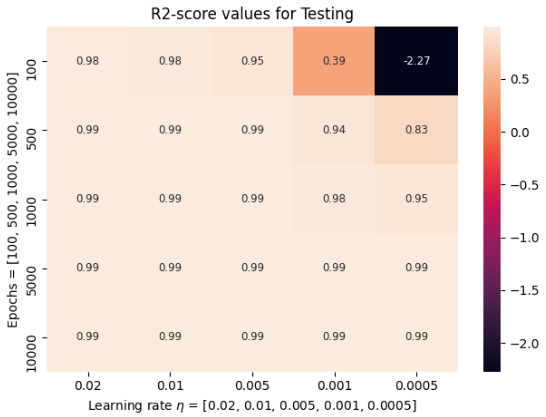
\includegraphics[width=7cm]{heatmapA2}
\caption{Heat-map containing the R2-score training and testing results of a Grid-Search with Learning rates = [0.02, 0.01, 0.005, 0.0001, 0.0005] and epochs = [100, 500, 1000, 5000, 10000].}
\end{figure}

As one can see, the design matrix ($\boldsymbol{X}$) with degree equals to 10 explains the response variable ($\boldsymbol{z}$) at a rate of 99 percent, according to the r2-scores in \hyperref[fig:figA1]{Fig.6}. In other words, these results suggest that the input polynomials translate almost entirely the output heights of the terrain region studied.

\begin{figure}[H]
\label{fig:figA2}
\centering
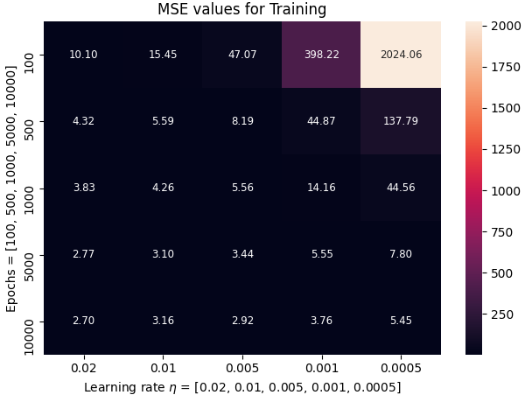
\includegraphics[width=7cm]{heatmapA3}
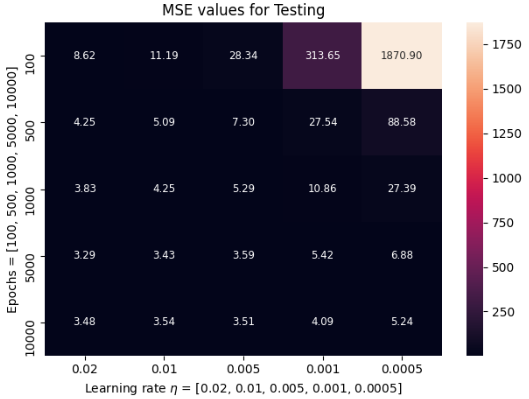
\includegraphics[width=7cm]{heatmapA4}
\caption{Heat-map containing the MSE training and testing results of a Grid-Search with Learning rates = [0.02, 0.01, 0.005, 0.0001, 0.0005] and epochs = [100, 500, 1000, 5000, 10000]. }
\end{figure}

The results from training and testing heat-maps \hyperref[fig:fidA2]{Fig.7} shows that the best testing MSE score is 2.99 for learning rates 0.02 and epochs 10.000. Notice that as the number of epochs increases, the MSE scores decreases indicating that the gradient of the loss-function is in the direction of the minimum local/global as expected. 

\begin{figure}[H]
\label{fig:figA3}
\centering
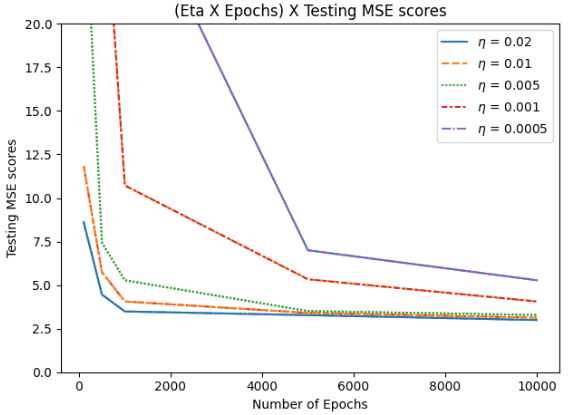
\includegraphics[height=5cm]{linesA1}
\caption{Line-plot showing (Eta x Epochs) X Testing MSE scores. }
\end{figure}

\hyperref[fig:figA3]{Fig.8} shows that the accuracy for learning rates 0.02, 0.01 and 0.005 converges to its best score near 1.000 epochs. Therefore, we choose the number of epochs equals 1.000 as the parameter's benchmarks on futures experiments.

\subsubsection{Tuning computation's cost (mini-batches)}
\label{chap:Tuning computation's cost (mini-batches)}

\qquad \, The SGD method with a unique mini-batch is costly for computations while fitting the model. The algorithm stochastically chooses a single vector of features from the sample space, calculates the gradient, and updates the weights. This process is repeated for as many samples in the design matrix ($\boldsymbol{X}$) for every epoch. It turns out that the number of computations sky rocks and the entire fitting takes a long time to complete, as shown on the heat-map below:

\begin{figure}[H]
\label{fig:figA4}
\centering
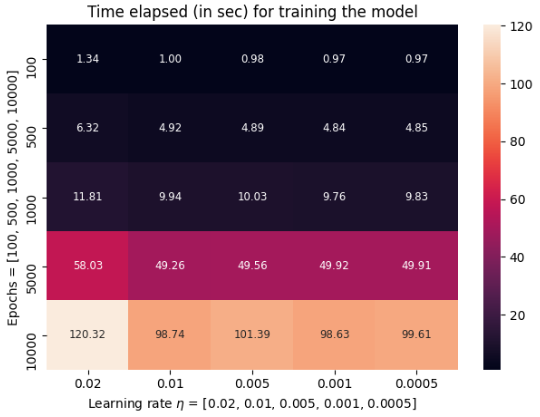
\includegraphics[width=8cm]{heatmapA5}
\caption{Heat-map containing the fitting time (in seconds) of the previous Grid-Search on \hyperref[fig:figA1]{Fig.1} and \hyperref[fig:figA2]{Fig.2}.}
\end{figure}

It is evident that as the number of epochs is high, the computations' costs are higher. For example, our model's fitting time takes approx. 1 seconds to run when the epoch number is 100. On the other hand, when the epoch is 10.000, the fitting time takes approx. 100 seconds.\\

To avoid the cost of this expensive computation, we introduce the mini-batches technique. Instead of stochastically choosing only one vector of features from the training sample, the algorithm chooses feature vectors blocks.\\

Therefore, we perform a Grid-Search for the parameters etas=[0.01, 0.005, 0.001, 0.0005] and batch\_sizes=[1, 5, 10, 15, 20], using our bench-marked epoch value equal 1.000, and analyse the testing MSE performance and fitting's time on the heat-maps below:

\begin{figure}[H]
\label{fig:figA5}
\centering
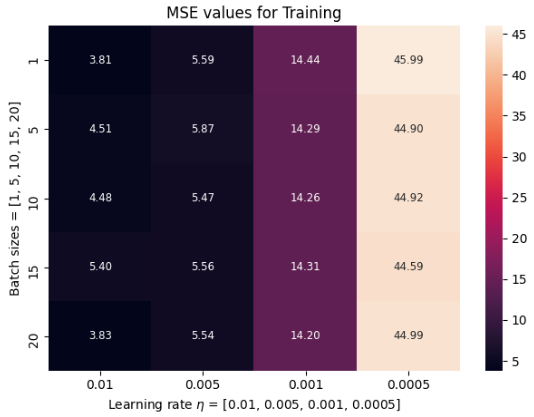
\includegraphics[width=7cm]{heatmapA6}
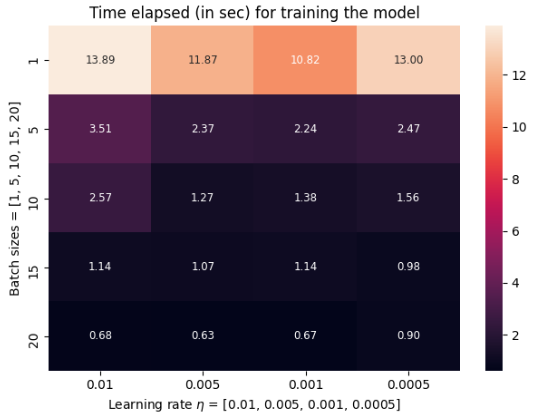
\includegraphics[width=7cm]{heatmapA7}
\caption{Left heat-map shows the testing MSE scores for each search. Right heat-map shows the fitting's time for each search.}
\end{figure}

For a single vector of features (batch\_size=1), the elapsed fitting's times are above 10 seconds. Under blocks of feature vectors (mini-batches), the elapsed fitting times have a tremendous reduction without losing much the accuracy. For example, the case with learning rate=0.01 and batch-size=1 got MSE equals 3.81, and fitting's time equals 13.89 seconds, however for the same learning rate=0.01, but batch\_size=20, the fitting's time was approx. 20 times faster and with almost the same accuracy of 3.83.

\begin{figure}[H]
\label{fig:figA6}
\centering
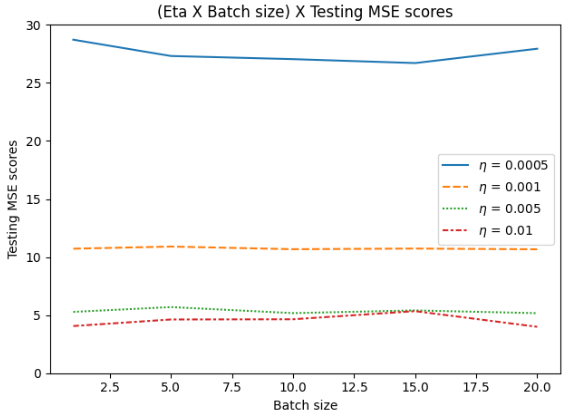
\includegraphics[height=5cm]{linesA2}
\caption{Line.plot containing (Eta x Batch size) X testing MSE.}
\end{figure}

\hyperref[fig:figA6]{Fig.11} shows that the constant learning rate $\eta$=0.01 performs better than the other learning rates. It has constant accuracy for all batch sizes tested. Besides, we see that batch\size=10 is the sweet spot for $\eta$=0.01 because it is where the accuracy starts to worsen.\\

Hence, we define our bench-marked parameters epochs=1.000 and batch\_size=10 for futures examinations.

\subsubsection{Learning rate decay and tuning decay}
\label{chap:Learning rate decay and tuning decay}

\qquad \, There are many ways to optimize the learning rate to find more accurate predictions. As studied in \hyperref[chap:Gradient Decedent]{Gradient Descent theory}, the learning rate ($\eta$) is a hyper-parameter that manages the model's change in response to the MSE each time the model's coefficients (weights) are updated.\\

Now, we apply a technique that reduces the learning rate value according to the number of epochs, studied in \hyperref[chap:Learning Rate with decay]{Learning rate decay}. To do that, we introduce a constant parameter called decay.\\

Thus, we run a Grid-Search with the parameters etas=[0.35, 0.3, 0.25, 0.2, 0.01] and decays=[10**-1, 10**-2, 10**-3, 10**-4, 10**-5], using our bench-marked epoch=1.000 and batch-size=10, to find the best testing MSE score for an eta as a function of a decay value:

\begin{figure}[H]
\label{fig:figA7}
\centering
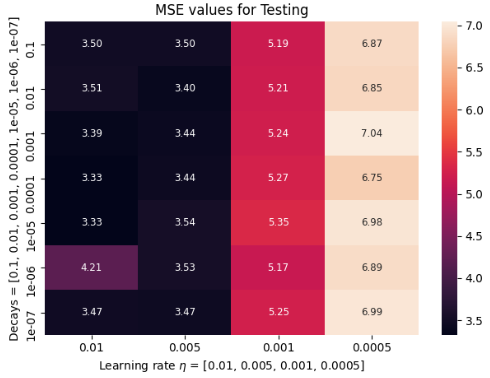
\includegraphics[height=5cm]{heatmapA8}
\caption{Heat-map showing the testing MSE scores for learning rates as function of decays.}
\end{figure}

With this decay technique, we were able to increase the learning rate without breaking the gradient calculation. Therefore, the best testing MSE achieved was 4.32 for learning rate=0.3 and decay=0.001.\\

Hence, we include decay=0.001 and eta0=0.3 to our bench-marked parameters epochs=1.000, batch\_size=10. We will try to beat the testing MSE of 4.32 obtained in this section by introducing mini-batch SGD momentum (gamma) and 'l2' regularization in the following sub-sections.

\subsubsection{SGD with momentum and tuning gamma}
\label{chap:SGD with momentum and tuning gamma}

\qquad \, This subsection will try to overcome the testing MSE of 4.32 by applying another type of Mini-batch Stochastic Gradient Descent, so-called Mini-batch SGD with momentum. A new parameter gamma is introduced, as explained in the theory section in \hyperref[chap:BGD, SGD and Mini-batch SGD with momentum]{"BGD, SGD and Mini-batch SGD with momentum"}. We use different values of gamma=[0, 0.1, 0.2, 0.25, 0.3, 0.35, 0.4, 0.5, 0.6] and run the model \href{https://github.com/fabiorodp/UiO-FYS-STK4155/blob/master/Project2/package/gradient_descent.py}{MiniSGDM} with the bench-marked parameters obtained from the previous subsections, decay=0.001, eta0=0.3, epochs=1.000 and batch\_size=10.

\begin{figure}[H]
\label{fig:figA8}
\centering
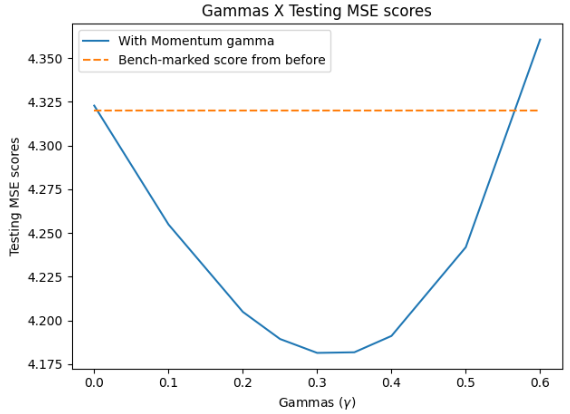
\includegraphics[width=7cm]{linesA3}
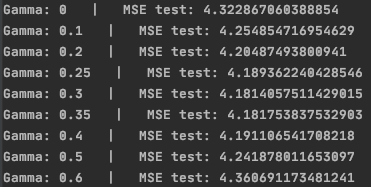
\includegraphics[width=7cm]{outputA1}
\caption{Left line-plot containing the MSE values as function of gammas. Right output of accuracy values for gammas.}
\end{figure}

As shown, the Mini-batch Stochastic Gradient Descent with momentum overcome our bench-marked score of 4.32, reaching 4.18 when gamma parameter is 0.3.\\

Hence, we include gamma=0.3 to our bench-marked parameters decay=0.001, eta0=0.3, epochs=1.000, batch\_size=10. We will try to beat the testing MSE of 4.1814 obtained in this section by introducing 'l2' regularization (Ridge lambda) in the next sub-section.

\subsubsection{'L2' regularization and tuning lambda}
\label{chap:'L2' regularization and tuning lambda}

\qquad \, This subsection will try to overcome the testing MSE of 3.65 by applying the l2 regularization (Ridge). A new parameter lambda is introduced, as explained in the theory section of \href{https://github.com/fabiorodp/UiO-FYS-STK4155/blob/master/Project1}{Project 1}. We use different values of lambda=[0, 10**-9, 10**-6, 10**-4] and run the model \href{https://github.com/fabiorodp/UiO-FYS-STK4155/blob/master/Project2/package/gradient_descent.py}{MiniSGDM} with the bench-marked parameters obtained from the previous subsections, gamma=0.3, decay=0.001, eta0=0.3, epochs=1.000 and batch\_size=10.

\begin{figure}[H]
\label{fig:figA9}
\centering
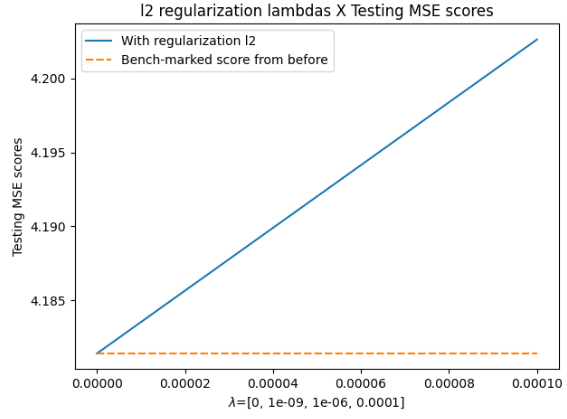
\includegraphics[width=8cm]{linesA4}
\caption{Line-plot containing the MSE values as function of lambdas.}
\end{figure}

As exhibited, the 'l2' regularization did not make any improvement overcoming our bench-marked testing accuracy of 4.1814.

\subsection{Part B and C}
\label{chap:Part B and C}

\qquad \, In part B and C of this report, we will discuss the application of our own Feed Forward Deep Neural Network (DNN) with the back-propagation method on a regression problem. The data-set applied on DNN will be the GeoTIF terrain image utilized in part A. It is essential to mention that the descriptive data-set will not be submitted to a design matrix function, as we did in part A, because the DNN should identify possible linearity by itself. Also, the targets will not be scaled, as we did not do that on "Project 1" and part A. These choices are because of comparisons propose as the performances between OLS, Ridge, Mini-batch SGDM and DNN will be distinguished, and we want to feed the models with almost the same complexities as fed before.\\

The cost-function employed is the Mean Squared Error (MSE) due to the regression nature of this kind of problem. Also, as explained on the \hyperref[chap:Deep Neural Networks]{DNN theory topic}, the MSE function matches very well on models that use gradient descent because of MSE's convexity and continuity aspects.\\

Moreover, the activation function for the hidden layers will be Sigmoid on the first experiments and then Tanh and Relu. The output layer's activation function will be "identity" because DNN for regression cases does not use an activation function for output values.\\

The way that the models' weights and biases are initialized is through Gaussian distribution, but another method so-called "Xavier" will be explored. Both approaches are explained in detail in the theory section.\\

Finally, the number of epochs tested in this section will be fixed at 500 because of computation costs. The batch\_size will also be fixed at the samples' length in training data due to the best metrics than mini-batches.

\subsubsection{Number of Neurons Vs Learning rates for 1 hidden-layer NN-MLP}
\label{chap:Number of Neurons Vs Learning rates for 1 hidden-layer NN-MLP}

\qquad \, At the beginning of part B of this report, we will employ a one-layer neural network to analyze different vital topics regarding the number of neurons, learning rate, epoch, cost error, decay, and 'l2' regularization.\\

The Python function called one\_hidden\_layer\_sigmoid at file \href{https://github.com/fabiorodp/UiO-FYS-STK4155/blob/master/Project2/partBandC.py}{partBandC.py} in the directory \href{https://github.com/fabiorodp/UiO-FYS-STK4155/blob/master/Project2/}{Project2/} will perform the following experiments and return the results we will discuss here.\\

First, we would like to find the best number of neurons as a function of a learning rate ($\eta$) value. For that, n\_neurons = [10, 20, 30, 40, 50, 75, 100, 125, 150] and etas = [0.99, 0.9, 0.8, 0.7, 0.6, 0.5] are defined and performed on our class SearchParametersDNN in \href{https://github.com/fabiorodp/UiO-FYS-STK4155/blob/master/Project2/package/studies.py}{studies.py} at directory \href{https://github.com/fabiorodp/UiO-FYS-STK4155/blob/master/Project2/package/}{package/}. This class method fits our Multi-layer perceptron (MLP) function with a combination of the previous parameters, one by one, to identify which one returns the best metrics as follows:

\begin{figure}[H]
\label{fig:B1}
\centering
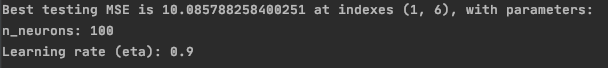
\includegraphics[width=12cm]{B1}
\caption{Output for printing best combination of metrics.}
\end{figure}

This first output shows that the best combination of parameters is neurons = 100 and learning rate = 0.9, which obtained testing MSE at 10.0857.

\begin{figure}[H]
\label{fig:B2}
\centering
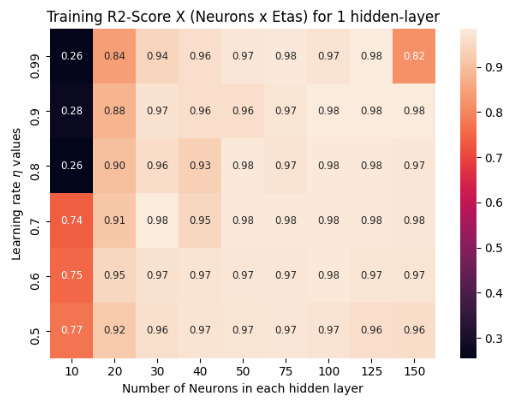
\includegraphics[height=5cm]{B2}
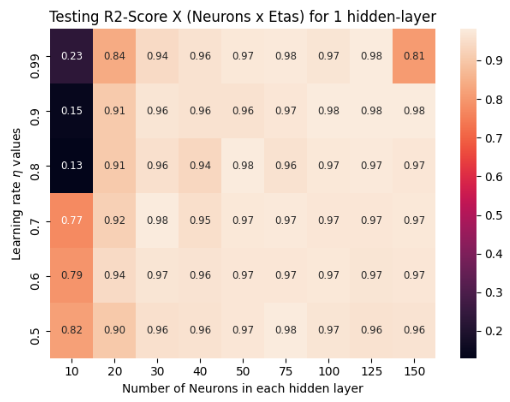
\includegraphics[height=5cm]{B3}
\caption{Heat-maps containing the R2-score training and testing results.}
\end{figure}

\begin{figure}[H]
\label{fig:B3}
\centering
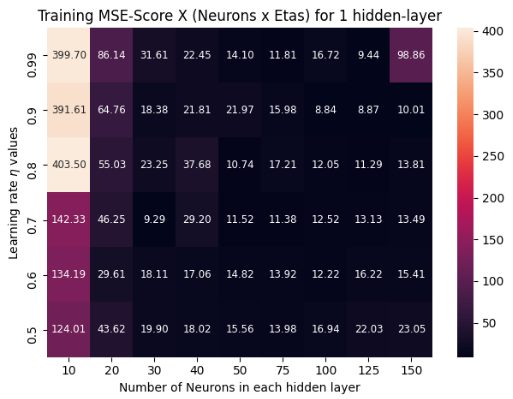
\includegraphics[height=5cm]{B4}
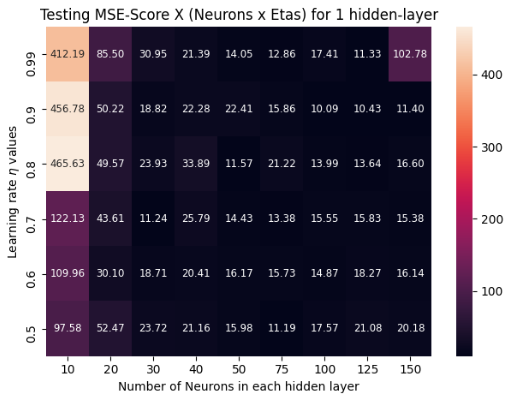
\includegraphics[height=5cm]{B5}
\caption{Heat-maps containing the MSE-score training and testing results.}
\end{figure}

The results are promising because the model reached r2-score around 99 percent for only one hidden-layer. The best training and testing MSE accuracies were 8.84 and 10.09, respectively, at neurons = 100 and $\eta$ = 0.9. Observe that when the neurons and learning rates are smaller or larger than 100 and 0.9, the model gets worse scores, indicating that the parameters are optimized.

\begin{figure}[H]
\label{fig:B4}
\centering
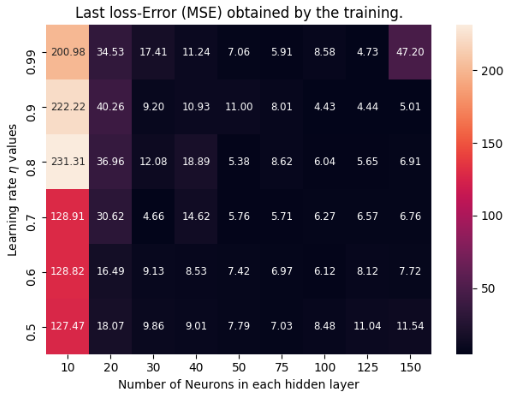
\includegraphics[height=5.5cm]{B6}
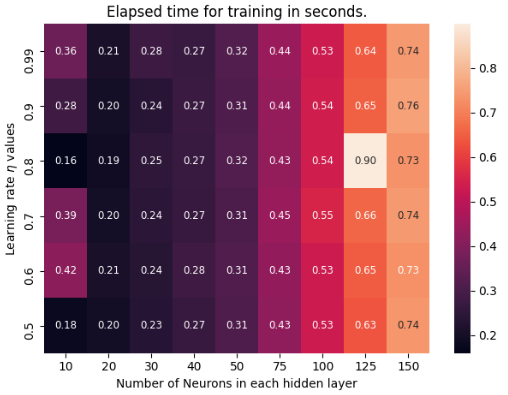
\includegraphics[height=5.5cm]{B7}
\caption{Heat-maps containing the loss-error for the last training epoch (left) and elapsed training times (right).}
\end{figure}

The loss-error is the MSE score measured for every Feed-Forward process for every epoch during training. As shown above, the best loss-error for the last training epoch at neurons = 100 and $\eta$=0.9 likewise was the smallest/best with a 4.43 score. This score is overestimated because the training and testing MSE scores were higher in \hyperref[fig:B3]{Figure 17}. Besides, as the number of neurons is high, the time elapsed for training is more considerable.

\begin{figure}[H]
\label{fig:B5}
\centering
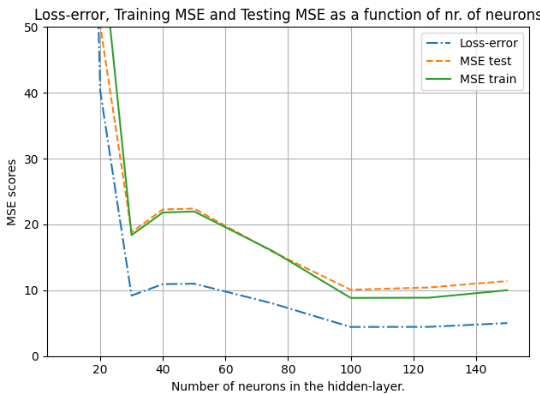
\includegraphics[height=5.5cm]{B8}
\caption{Line-plot containing the loss-error, training and testing MSE scores for $\eta$=0.9 and different neurons values.}
\end{figure}

\hyperref[fig:B5]{The previous figure} shows that our parameter's sweet spot is 100 for the number of neurons. This parameter is optimal because it reached the best score in the searching and where the bias and variance of the model are the lowest since loss-error, training and testing lines are in the smallest score and closest among each other. Besides, an increase in the variance happens when the complexity number of neurons increases above 100, where the scores worsen, and the difference among loss-error, training and testing increases.

\subsubsection{Accuracy analysis and epochs analysis}
\label{chap:Accuracy analysis and epochs analysis}

\qquad \, Considering our best model from the previous sub-topic, we can analyze each epoch's accuracy score's evolution by the succeeding line-plots:

\begin{figure}[H]
\label{fig:B6}
\centering
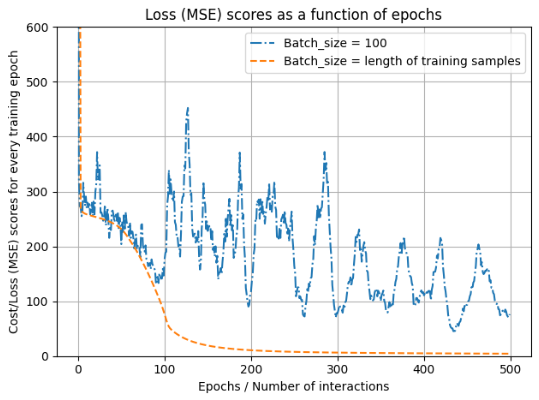
\includegraphics[height=5.5cm]{B9}
\caption{Line-plot containing the cost/loss-error for every training epoch.}
\end{figure}

At the beginning of the fitting, the accuracy is terrible because of the randomness initiation of the layers' weights and biases. As long as the epochs are processed, our gradient descent does an excellent task, converging and decreasing to the local or global minimum score.\\

It is imperative to say that we were using the parameter batch\_size equals the number of samples of the training data. This parameter makes the cost curve above being smooth due to the batch gradient descent essence, as explained in theory.\\

However, when we define batch\_size equals 100, less than the number of samples of the training data, then the cost curve will differ, being choppy due to the Stochastically nature of the mini-batches choices. Nonetheless, the gradient descent still performs very well, converging the cost to its minimum as expected. This option of batch\_size gains a lot in speedy of the computation, likewise explained at \hyperref[chap:Tuning computation's cost (mini-batches)]{part A - "Tuning computation's cost (mini-batches)"}, and it is ideal for extensive explanatory data with a considerable number of samples and features.

\subsubsection{Tuning the learning rate, decay and "l2" regularization}
\label{chap:Tuning the learning rate, decay and "l2" regularization}

\qquad \, We will tune the parameters learning rate ($\eta$), decay and 'l2' Ridge regularization lambda. Remember that the explanations about each parameter are in the theory section. For this optimization, we choose different values for etas = [0.99, 0.95, 0.9, 0.85, 0.8, 0.7, 0.6, 0.5], decays = [0, 10 ** -9, 10 ** -8, 10 ** -7, 10 ** -6, 10 ** -5, 10 ** -4, 10 ** -3, 10 ** -2, 10 ** -1] and lambdas = [0, 10 ** -9, 10 ** -8, 10 ** -7, 10 ** -6, 10 ** -5, 10 ** -4, 10 ** -3, 10 ** -2, 10 ** -1], and then perform the MLP model for each combination of parameters. The printed output shows the best parameters and testing MSE score for the best combination:

\begin{figure}[H]
\label{fig:B7}
\centering
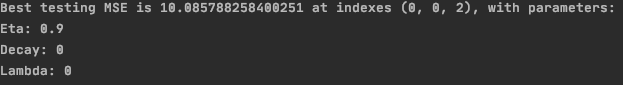
\includegraphics[width=12cm]{B10}
\caption{Printed output containing the best parameters of the searching.}
\end{figure}

This output confirms that the learning rate equal to 0.9 acquired before is optimized. Besides, the decay and lambda parameters did not help the MLP model overcome the testing MSE score of 10.085.

\begin{figure}[H]
\label{fig:B8}
\centering
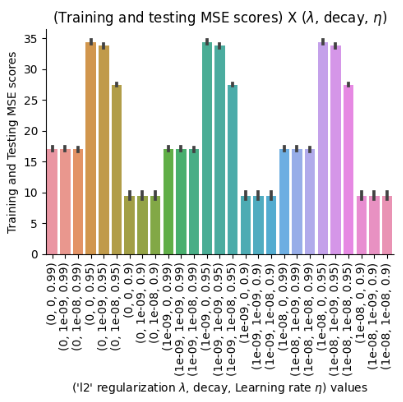
\includegraphics[height=8cm]{B11}
\caption{Bar-plot containing selected best scores for the $\eta$, decay and $\lambda$ parameter search. The upper extreme of the black bars is the testing MSE scores, and the lower extreme of the same black bars is the training MSE scores. The colored bars are the average between training and testing MSE scores.}
\end{figure}

The \hyperref[fig:B8]{bar-plotting above} shows that the 'l2' regularization and decay did not produce any furtherance in the best score. Although, parameters ($\lambda$=1e-9, decay=1e-9, $\eta$=0.9) and ($\lambda$=1e-8, decay=1e-8, $\eta$=0.9) achieved pretty close scores to ($\lambda$=0, decay=0, $\eta$=0.9). Since $\lambda$ attenuates the variance and avoids over-estimations and over-fitting of the model, those sets of parameters with $\lambda$ different from 0 might be better choice.

\begin{figure}[H]
\label{fig:B9}
\centering
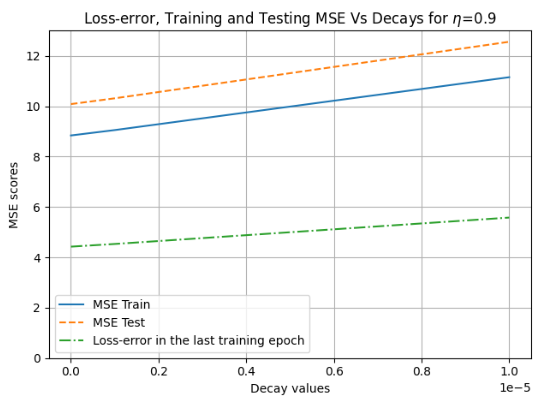
\includegraphics[height=5.5cm]{B12}
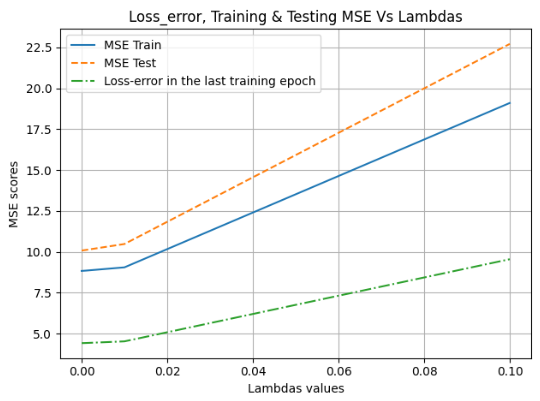
\includegraphics[height=5.5cm]{B13}
\caption{Line-plots containing loss-error, training and testing MSE as a function of decays (left), loss-error, training and testing MSE as a function of lambdas (right).}
\end{figure}

The \hyperref[fig:B9]{line-plots above} confirm that the MSE scores did not improve by applying decay and lambda parameters.

\subsubsection{Terrain image data on 2 hidden-layers MLP-DNN}
\label{chap:Terrain image data on 2 hidden-layers MLP-DNN}

\subsubsection{Tanh activation function}
\label{chap:Tanh activation function}

\subsubsection{ReLu activation function}
\label{chap:ReLu activation function}

\subsubsection{Initializing weights and biases by Xavier method}
\label{chap:Initializing weights and biases by Xavier method}

\subsection{Part D}
\label{chap:Part D}

\subsection{Part E}
\label{chap:Part E}

